% How the global random state takes part when a function draws in the body of
% nv_scan(): the function; the graph jit() traces from it, with the part that
% implements the random state in blue; the views of the random state in the
% program's trace and in the body's; the host object; and numbered notes on
% what happens.
% Build: see figures/README.md
\documentclass[tikz, border = 6pt]{standalone}
\usepackage[T1]{fontenc}
\usepackage{lmodern}
\usetikzlibrary{positioning, calc, fit, backgrounds, matrix}

\definecolor{keep}{HTML}{2A7AB0}

% The part of the graph that implements the side effect, and the part of it
% that is not used.
\newcommand{\se}[1]{\textcolor{keep}{#1}}
\newcommand{\unused}[1]{\textcolor{black!40}{#1}}
% An annotation next to a line of the graph.
\newcommand{\aside}[1]{\hspace{1.5em}{\normalfont\sffamily\itshape\color{black!60}$\leftarrow$ #1}}
\newcommand{\cd}[1]{\texttt{#1}}

\tikzset{
  badge/.style = {circle, fill = black!65, text = white, font = \sffamily\tiny\bfseries,
    inner sep = 0pt, minimum size = 3.2mm, anchor = base},
  lines/.style = {matrix of nodes, row sep = {3.9mm, between origins}, column sep = 2pt,
    nodes = {anchor = base west, inner sep = 0.5pt, font = \ttfamily\scriptsize},
    column 2/.style = {nodes = {badge}}, column 3/.style = {nodes = {badge}}},
  fields/.style = {matrix of nodes, row sep = {3.9mm, between origins}, column sep = 2pt,
    nodes = {anchor = base west, inner sep = 0.5pt, font = \ttfamily\scriptsize},
    column 1/.style = {nodes = {text = black!55}}},
  box/.style = {rounded corners = 2pt, inner sep = 5pt},
  head/.style = {font = \footnotesize\bfseries, text = black!70, anchor = south west,
    inner sep = 1pt},
  note/.style = {font = \footnotesize, align = left, text width = 8.6cm, anchor = north west,
    inner sep = 0pt, execute at begin node = {\thickmuskip = 5mu}}
}

% A note: its text at #2, numbered #1 in a badge hanging to its left.
\newcommand{\note}[3]{
  \node[note] (#1) at #2 {#3};
  \node[badge, font = \sffamily\scriptsize\bfseries, minimum size = 3.8mm, anchor = north east]
    at ($(#1.north west) + (-0.15, 0.04)$) {#1};
}

\begin{document}
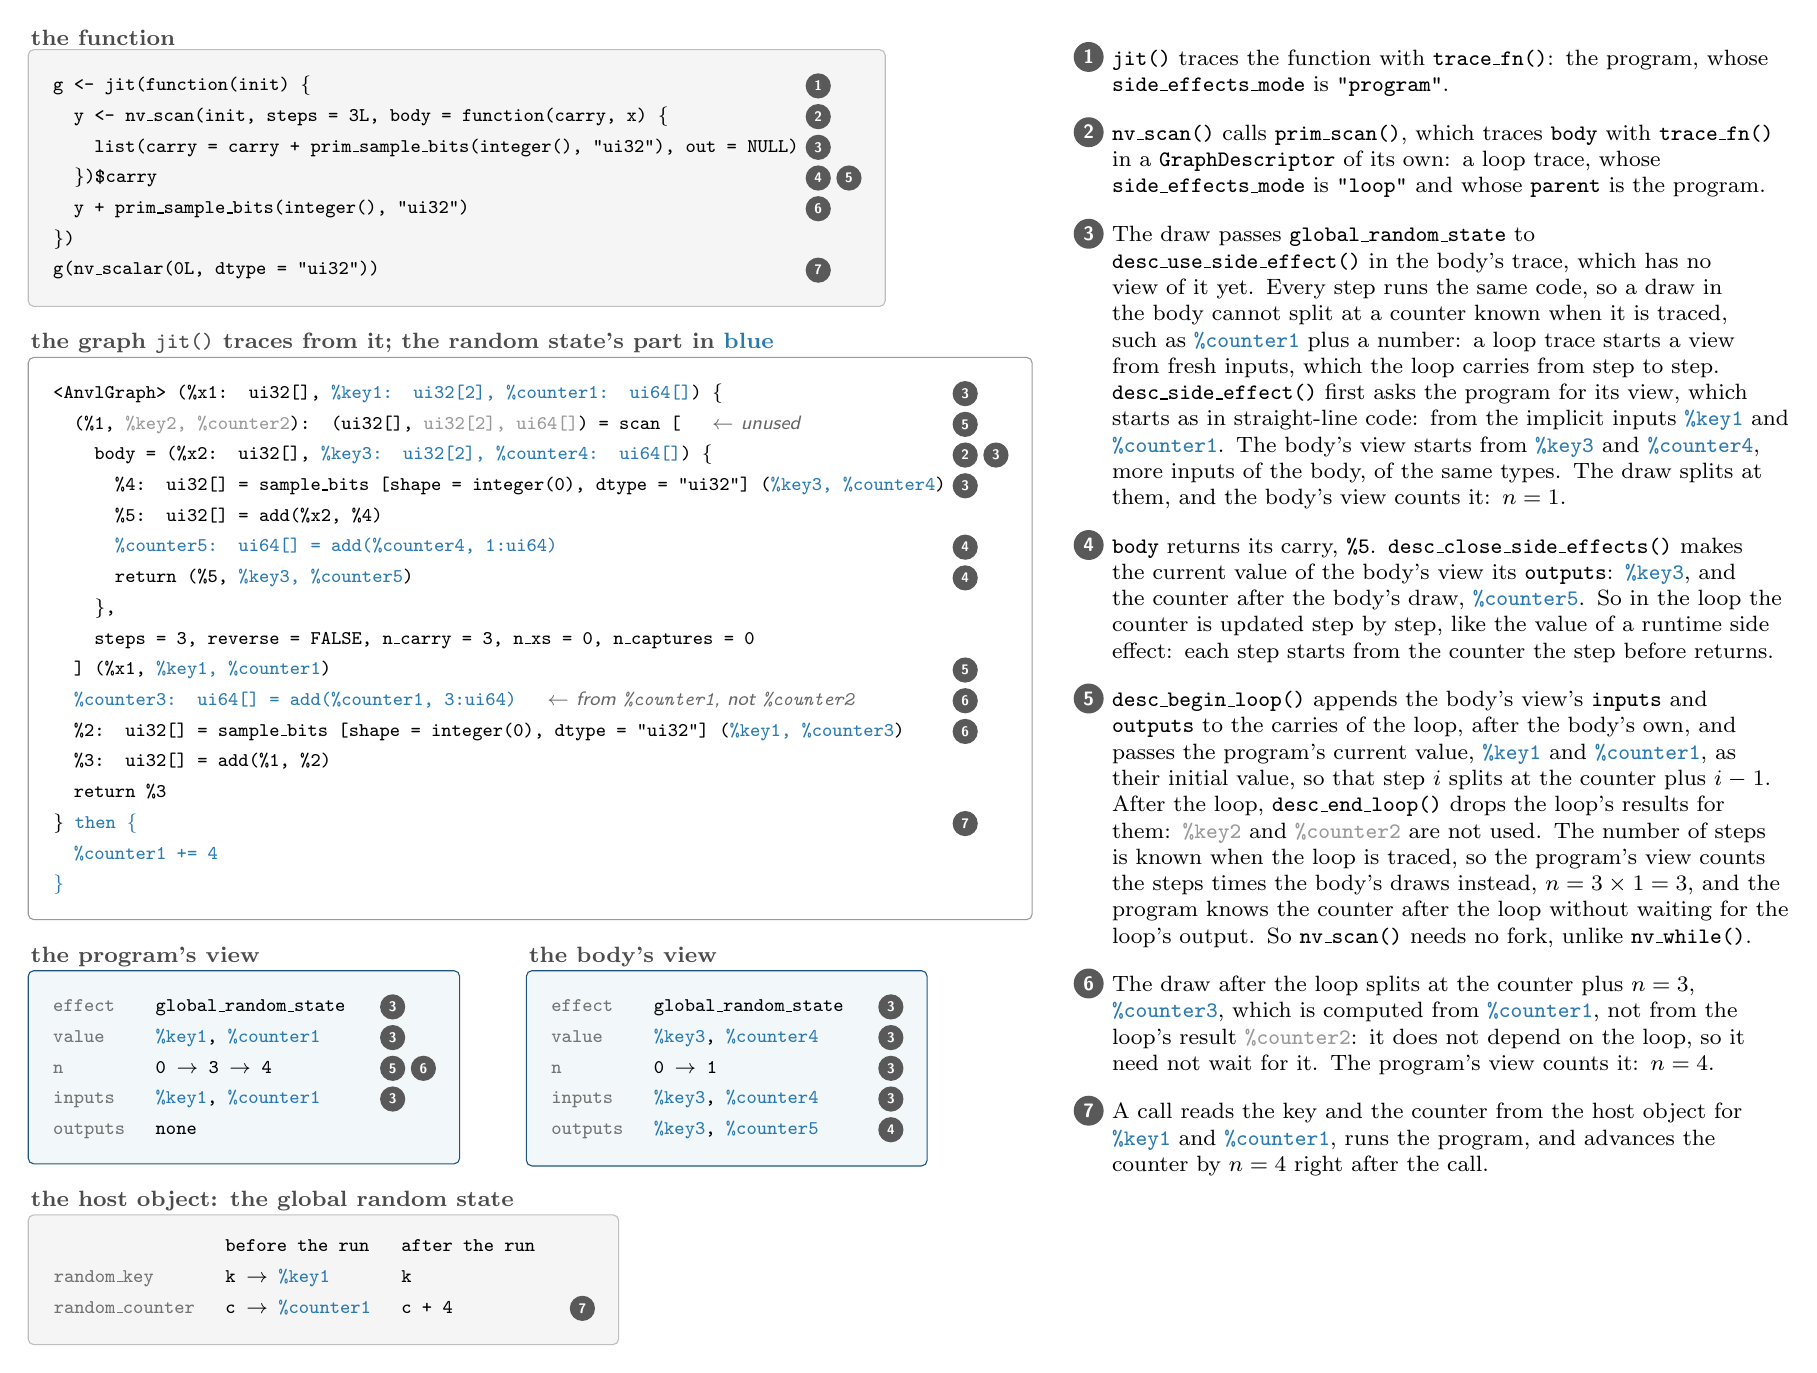
\begin{tikzpicture}

  \matrix[lines] (code) at (0, 0) {
    g <- jit(function(init) \{ & 1 \\
    \ \ y <- nv\_scan(init, steps = 3L, body = function(carry, x) \{ & 2 \\
    \ \ \ \ list(carry = carry + prim\_sample\_bits(integer(), "ui32"), out = NULL) & 3 \\
    \ \ \})\$carry & 4 & 5 \\
    \ \ y + prim\_sample\_bits(integer(), "ui32") & 6 \\
    \}) & \\
    g(nv\_scalar(0L, dtype = "ui32")) & 7 \\
  };
  \begin{scope}[on background layer]
    \node[box, draw = black!25, fill = black!4, fit = (code)] (codebox) {};
  \end{scope}
  \node[head] at (codebox.north west) {the function};

  \matrix[lines, below = 1.0 of code.south west, anchor = north west] (graph) {
    <AnvlGraph> (\%x1: ui32[], \se{\%key1: ui32[2], \%counter1: ui64[]}) \{ & 3 \\
    \ \ (\%1, \unused{\%key2, \%counter2}): (ui32[], \unused{ui32[2], ui64[]}) = scan [\aside{unused} & 5 \\
    \ \ \ \ body = (\%x2: ui32[], \se{\%key3: ui32[2], \%counter4: ui64[]}) \{ & 2 & 3 \\
    \ \ \ \ \ \ \%4: ui32[] = sample\_bits [shape = integer(0), dtype = "ui32"] (\se{\%key3, \%counter4}) & 3 \\
    \ \ \ \ \ \ \%5: ui32[] = add(\%x2, \%4) & \\
    \ \ \ \ \ \ \se{\%counter5: ui64[] = add(\%counter4, 1:ui64)} & 4 \\
    \ \ \ \ \ \ return (\%5, \se{\%key3, \%counter5}) & 4 \\
    \ \ \ \ \}, & \\
    \ \ \ \ steps = 3, reverse = FALSE, n\_carry = 3, n\_xs = 0, n\_captures = 0 & \\
    \ \ ] (\%x1, \se{\%key1, \%counter1}) & 5 \\
    \ \ \se{\%counter3: ui64[] = add(\%counter1, 3:ui64)}\aside{from \texttt{\%counter1}, not \texttt{\%counter2}} & 6 \\
    \ \ \%2: ui32[] = sample\_bits [shape = integer(0), dtype = "ui32"] (\se{\%key1, \%counter3}) & 6 \\
    \ \ \%3: ui32[] = add(\%1, \%2) & \\
    \ \ return \%3 & \\
    \} \se{then \{} & 7 \\
    \ \ \se{\%counter1 += 4} & \\
    \se{\}} & \\
  };
  \begin{scope}[on background layer]
    \node[box, draw = black!40, fit = (graph)] (graphbox) {};
  \end{scope}
  \node[head] at (graphbox.north west)
    {the graph \cd{jit()} traces from it; the random state's part in \se{blue}};

  \matrix[fields, below = 1.0 of graph.south west, anchor = north west] (pview) {
    effect &[8pt] global\_random\_state &[10pt] |[badge]| 3 \\
    value & \se{\%key1}, \se{\%counter1} & |[badge]| 3 \\
    n & 0 $\to$ 3 $\to$ 4 & |[badge]| 5 & |[badge]| 6 \\
    inputs & \se{\%key1}, \se{\%counter1} & |[badge]| 3 \\
    outputs & none \\
  };
  \begin{scope}[on background layer]
    \node[box, draw = keep!70!black, fill = keep!6, fit = (pview)] (pviewbox) {};
  \end{scope}
  \node[head] at (pviewbox.north west) {the program's view};

  \matrix[fields, anchor = north west] (bview) at ($(pview.north east) + (1.2, 0)$) {
    effect &[8pt] global\_random\_state &[10pt] |[badge]| 3 \\
    value & \se{\%key3}, \se{\%counter4} & |[badge]| 3 \\
    n & 0 $\to$ 1 & |[badge]| 3 \\
    inputs & \se{\%key3}, \se{\%counter4} & |[badge]| 3 \\
    outputs & \se{\%key3}, \se{\%counter5} & |[badge]| 4 \\
  };
  \begin{scope}[on background layer]
    \node[box, draw = keep!70!black, fill = keep!6, fit = (bview)] (bviewbox) {};
  \end{scope}
  \node[head] at (bviewbox.north west) {the body's view};

  \matrix[fields, below = 1.0 of pview.south west, anchor = north west] (host) {
    &[8pt] before the run &[8pt] after the run \\
    random\_key & k $\to$ \se{\%key1} & k \\
    random\_counter & c $\to$ \se{\%counter1} & c + 4 &[10pt] |[badge]| 7 \\
  };
  \begin{scope}[on background layer]
    \node[box, draw = black!25, fill = black!4, fit = (host)] (hostbox) {};
  \end{scope}
  \node[head] at (hostbox.north west) {the host object: the global random state};

  \coordinate (notes) at ($(codebox.north -| graphbox.east) + (1.0, 0)$);
  \note{1}{(notes)}
    {\cd{jit()} traces the function with \cd{trace\_fn()}: the program, whose
     \cd{side\_effects\_mode} is \cd{"program"}.}
  \note{2}{($(1.south west) + (0, -0.35)$)}
    {\cd{nv\_scan()} calls \cd{prim\_scan()}, which traces \cd{body} with \cd{trace\_fn()} in a
     \cd{GraphDescriptor} of its own: a loop trace, whose \cd{side\_effects\_mode} is
     \cd{"loop"} and whose \cd{parent} is the program.}
  \note{3}{($(2.south west) + (0, -0.35)$)}
    {The draw passes \cd{global\_random\_state} to \cd{desc\_use\_side\_effect()} in the
     body's trace, which has no view of it yet. Every step runs the same code, so a draw in
     the body cannot split at a counter known when it is traced, such as \se{\cd{\%counter1}}
     plus a number: a loop trace starts a view from fresh inputs, which the loop carries from
     step to step. \cd{desc\_side\_effect()} first asks the program for its view, which
     starts as in straight-line code: from the implicit inputs \se{\cd{\%key1}} and
     \se{\cd{\%counter1}}. The body's view starts from \se{\cd{\%key3}} and
     \se{\cd{\%counter4}}, more inputs of the body, of the same types. The draw splits at
     them, and the body's view counts it: $n = 1$.}
  \note{4}{($(3.south west) + (0, -0.35)$)}
    {\cd{body} returns its carry, \cd{\%5}. \cd{desc\_close\_side\_effects()} makes the
     current value of the body's view its \cd{outputs}: \se{\cd{\%key3}}, and the counter
     after the body's draw, \se{\cd{\%counter5}}. So in the loop the counter is updated step
     by step, like the value of a runtime side effect: each step starts from the counter the
     step before returns.}
  \note{5}{($(4.south west) + (0, -0.35)$)}
    {\cd{desc\_begin\_loop()} appends the body's view's \cd{inputs} and \cd{outputs} to the
     carries of the loop, after the body's own, and passes the program's current value,
     \se{\cd{\%key1}} and \se{\cd{\%counter1}}, as their initial value, so that step $i$
     splits at the counter plus $i - 1$. After the loop, \cd{desc\_end\_loop()} drops the
     loop's results for them: \unused{\cd{\%key2}} and \unused{\cd{\%counter2}} are not used.
     The number of steps is known when the loop is traced, so the program's view counts the
     steps times the body's draws instead, $n = 3 \times 1 = 3$, and the program knows the
     counter after the loop without waiting for the loop's output. So \cd{nv\_scan()} needs no
     fork, unlike \cd{nv\_while()}.}
  \note{6}{($(5.south west) + (0, -0.35)$)}
    {The draw after the loop splits at the counter plus $n = 3$, \se{\cd{\%counter3}}, which
     is computed from \se{\cd{\%counter1}}, not from the loop's result
     \unused{\cd{\%counter2}}: it does not depend on the loop, so it need not wait for it.
     The program's view counts it: $n = 4$.}
  \note{7}{($(6.south west) + (0, -0.35)$)}
    {A call reads the key and the counter from the host object for \se{\cd{\%key1}} and
     \se{\cd{\%counter1}}, runs the program, and advances the counter by $n = 4$ right
     after the call.}

\end{tikzpicture}
\end{document}
